\section{Illustration}\label{sec:illustration}

Consider a sharp RDD with running variable $X$ (cutoff at $X = 0$) and a single continuous covariate $Z$.
The researcher observes $n = 6$ units at fixed design points $u_i = (x_i, z_i) \in [-1,1]^2$, $i = 1, \ldots, 6$, with outcomes
\begin{equation*}
	Y_i = m(u_i) + \varepsilon_i, \qquad \varepsilon_i \sim (0, \sigma^2),
\end{equation*}
where $m : [-1,1]^2 \to \mathbb{R}$ is the conditional expectation function and the target is $\tau = \lim_{x \downarrow 0} m(x,z) - \lim_{x \uparrow 0} m(x,z)$.
The design is arranged asymmetrically around the cutoff:

\begin{figure}[ht]
\centering
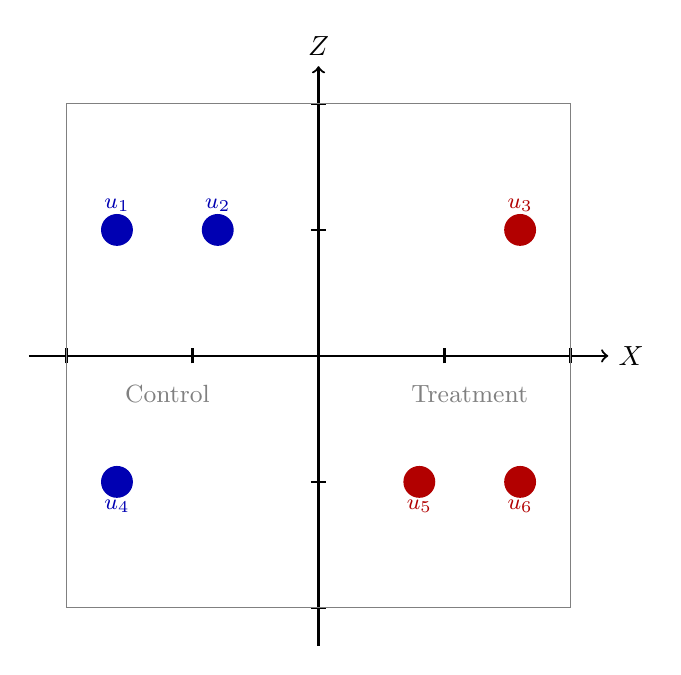
\begin{tikzpicture}[scale=3.2]

	% --- Coordinate axes ---
	\draw[->, thick] (-1.15, 0) -- (1.15, 0) node[right] {$X$};
	\draw[->, thick] (0, -1.15) -- (0, 1.15) node[above] {$Z$};

	% --- Tick marks ---
	\foreach \x in {-1, -0.5, 0.5, 1} {
		\draw[thick] (\x, -0.03) -- (\x, 0.03);
	}
	\foreach \z in {-1, -0.5, 0.5, 1} {
		\draw[thick] (-0.03, \z) -- (0.03, \z);
	}

	% --- Bounding box ---
	\draw[gray, thin] (-1,-1) rectangle (1,1);

	% --- Region labels ---
	\node[gray, font=\small] at (-0.6, -0.15) {Control};
	\node[gray, font=\small] at (0.6, -0.15) {Treatment};

	% --- Sample units ---
	% Top row: z = 0.5
	\fill[blue!70!black] (-0.8, 0.5) circle (1.8pt);
	\fill[blue!70!black] (-0.4, 0.5) circle (1.8pt);
	\fill[red!70!black] (0.8, 0.5) circle (1.8pt);

	% Bottom row: z = -0.5
	\fill[blue!70!black] (-0.8, -0.5) circle (1.8pt);
	\fill[red!70!black] (0.4, -0.5) circle (1.8pt);
	\fill[red!70!black] (0.8, -0.5) circle (1.8pt);

	% --- Unit labels ---
	\node[above=3pt, blue!70!black, font=\footnotesize] at (-0.8, 0.5) {$u_1$};
	\node[above=3pt, blue!70!black, font=\footnotesize] at (-0.4, 0.5) {$u_2$};
	\node[above=3pt, red!70!black, font=\footnotesize] at (0.8, 0.5) {$u_3$};

	\node[below=3pt, blue!70!black, font=\footnotesize] at (-0.8, -0.5) {$u_4$};
	\node[below=3pt, red!70!black, font=\footnotesize] at (0.4, -0.5) {$u_5$};
	\node[below=3pt, red!70!black, font=\footnotesize] at (0.8, -0.5) {$u_6$};

\end{tikzpicture}
\caption{Fixed design with $n = 6$ units. Control units (blue, $x_i < 0$) and treatment units (red, $x_i > 0$) are arranged in two rows at $z = \pm\tfrac{1}{2}$. The design is asymmetric: at $z = \tfrac{1}{2}$, two control units lie near the cutoff while only one treatment unit is available; at $z = -\tfrac{1}{2}$, the pattern reverses.}
\label{fig:design}
\end{figure}

The researcher knows that the partial derivatives of $m$ are bounded:
\begin{equation*}
	\abs{\frac{\partial m}{\partial x}} \leq M_x, \qquad \abs{\frac{\partial m}{\partial z}} \leq M_z.
\end{equation*}
These are the primitive smoothness bounds.
Without further assumptions on how $\partial m / \partial x$ and $\partial m / \partial z$ interact, the researcher faces a choice between two function classes that are both consistent with this information:

\begin{enumerate}
	\item The \emph{anisotropic class} $\mathcal{F}_1^{\mathrm{aniso}}(M_x, M_z)$ constrains each partial derivative independently.
	Its gradient constraint set is the rectangle $[-M_x, M_x] \times [-M_z, M_z]$: any combination of slopes $(\partial m / \partial x,\, \partial m / \partial z)$ satisfying the marginal bounds is permitted.
	This is the coupling-agnostic class (\cref{def:coupling_agnostic}).

	\item The \emph{isotropic class} $\mathcal{F}_1^{\mathrm{iso}}\!\bigl(\sqrt{M_x^2 + M_z^2}\bigr)$ constrains the gradient norm: $\norm{\nabla m}_2 \leq \sqrt{M_x^2 + M_z^2}$.
	Its gradient constraint set is the disk of radius $R = \sqrt{M_x^2 + M_z^2}$, which is the smallest disk containing the rectangle.
	This class imposes coupling (\cref{def:coupling}): it permits gradient pairs outside the rectangle (e.g., $(R, 0)$ with $R > M_x$) while forbidding pairs inside it (e.g., $(M_x, M_z)$ lies on the boundary of the disk but the disk extends beyond the rectangle along the axes).
\end{enumerate}

Since $\mathcal{F}_1^{\mathrm{aniso}}(M_x, M_z) \subsetneq \mathcal{F}_1^{\mathrm{iso}}\!\bigl(\sqrt{M_x^2 + M_z^2}\bigr)$, any estimator's worst-case risk is weakly lower under the anisotropic class.
The question is whether this improvement is strict, and how large it is in this concrete design.

\paragraph{Estimators.}
The local constant estimator assigns equal weight to all units on each side of the cutoff:
\begin{equation}\label{eq:lc_estimator}
	\hat\tau_{\mathrm{lc}} = \underbrace{\tfrac{1}{3}(Y_3 + Y_5 + Y_6)}_{\bar{Y}_T} - \underbrace{\tfrac{1}{3}(Y_1 + Y_2 + Y_4)}_{\bar{Y}_C}.
\end{equation}
Since both groups have size three, the difference of means can be written as the average of any complete matching between treatment and control units.
A natural matching pairs the closest units within each row and matches the remaining units across rows:
\begin{alignat*}{3}
	&\text{Upper pair:}  &\quad& (u_3, u_2): &\quad& \Delta_1 = u_3 - u_2 = (1.2,\; 0), \\
	&\text{Lower pair:}  &\quad& (u_5, u_4): &\quad& \Delta_2 = u_5 - u_4 = (1.2,\; 0), \\
	&\text{Cross pair:}  &\quad& (u_6, u_1): &\quad& \Delta_3 = u_6 - u_1 = (1.6,\; {-1}).
\end{alignat*}
The upper and lower pairs compare units at the same covariate value $z$, so their displacement vectors are purely horizontal.
The cross pair --- forced by the design asymmetry --- compares units at different covariate values, producing a displacement with both an $x$- and a $z$-component.
This cross pair is where the distinction between the anisotropic and isotropic classes matters.

The second estimator adjusts for the covariate by including stratum fixed effects --- one for the upper row ($z = \tfrac{1}{2}$) and one for the lower row ($z = -\tfrac{1}{2}$).
Within each stratum, it estimates a separate treatment effect and averages:
\begin{equation}\label{eq:seg_estimator}
	\hat\tau_{\mathrm{seg}} = \frac{1}{2}\underbrace{\Bigl[Y_3 - \tfrac{1}{2}(Y_1 + Y_2)\Bigr]}_{\hat\tau_{\mathrm{upper}}} + \frac{1}{2}\underbrace{\Bigl[\tfrac{1}{2}(Y_5 + Y_6) - Y_4\Bigr]}_{\hat\tau_{\mathrm{lower}}}.
\end{equation}
These are the weights implied by regressing $Y_i$ on a treatment indicator and a stratum fixed effect.
In the upper stratum, with two control units and one treatment unit, the control units each receive weight $\tfrac{1}{4}$ while the treatment unit receives weight $\tfrac{1}{2}$; in the lower stratum the pattern reverses.

The segmented estimator decomposes into four within-stratum pairs:
\begin{alignat*}{3}
	&\text{Upper:}  &\quad& (u_3, u_1), \; (u_3, u_2): &\quad& \Delta = (1.6,\; 0), \;\; (1.2,\; 0), \\
	&\text{Lower:}  &\quad& (u_5, u_4), \; (u_6, u_4): &\quad& \Delta = (1.2,\; 0), \;\; (1.6,\; 0).
\end{alignat*}
Every displacement vector is purely horizontal.
By comparing only within strata, the segmented estimator eliminates the cross-row pair entirely: the $z$-component never enters the bias.

\paragraph{Worst-case bias.}
The bias of a linear estimator $\hat\tau = \sum_i w_i Y_i$ is $\E[\hat\tau \given u_1, \ldots, u_6] - \tau = \sum_i w_i m(u_i) - \tau$.
The worst-case bias is the supremum of this expression over all $m$ in the function class.
By a multivariate mean value argument, the difference $m(u_i) - m(u_j)$ between any two design points is bounded by the directional Lipschitz constant along their displacement $u_i - u_j$.
Under the anisotropic class, this bound is $M_x \abs{x_i - x_j} + M_z \abs{z_i - z_j}$; under the isotropic class, it is $R \norm{u_i - u_j}_2$.

To isolate the phenomenon, set $M_x = 0$ and $M_z > 0$.
Under the anisotropic class, every function is constant in $x$: the gradient constraint set collapses from the rectangle $[-M_x, M_x] \times [-M_z, M_z]$ to the line segment $\{0\} \times [-M_z, M_z]$.
This has immediate consequences for both estimators:

\begin{itemize}
	\item \emph{Segmented estimator.}
	All four displacement vectors are purely horizontal.
	Since $m$ is constant in $x$, every within-stratum comparison has zero bias: $m(u_3) = m(u_2) = m(u_1)$ and $m(u_5) = m(u_6) = m(u_4)$.
	The segmented estimator is \emph{exactly unbiased} under the anisotropic class.
	Worst-case risk reduces to variance alone --- a parametric rate.

	\item \emph{Local constant estimator.}
	The within-row pairs $(u_3, u_2)$ and $(u_5, u_4)$ contribute zero bias, just as for the segmented estimator.
	But the cross pair $(u_6, u_1)$ compares units at $z = -\tfrac{1}{2}$ and $z = \tfrac{1}{2}$: the $z$-displacement survives.
	The worst-case function sets $m(x, z) = M_z \cdot z$, yielding bias $\tfrac{1}{3} M_z$.
\end{itemize}

Under the isotropic class with $M_x = 0$, the radius is $R = M_z$, but the class still permits variation in $x$: the gradient norm constraint $\norm{\nabla m}_2 \leq M_z$ allows the adversary to tilt the function along $x$ at the expense of $z$-variation.
The worst-case function concentrates non-smoothness in whatever direction the estimator's displacements point.
The information that $M_x = 0$ is present in the primitive bounds, but the isotropic class cannot encode it: the $\ell_2$ norm couples the two directions, so the direction-specific bound is not available to exploit.

\commentT{Compute explicit worst-case bias for both estimators under iso with $M_x = 0$. If needed, adjust design coordinates to obtain exact equality between the two estimators under the isotropic class.}

The extreme case $M_x = 0$ makes the mechanism transparent, but the logic extends to any $M_x > 0$.
The segmented estimator exploits the direction-specific bounds by confining comparisons to within-stratum pairs, eliminating the $z$-contribution from cross-stratum comparisons.
Under the anisotropic class, which encodes the bound $M_x = 0$ separately, this eliminates bias entirely.
Under the isotropic class, the adversary compensates by reallocating gradient budget into the $x$-direction, and the improvement vanishes or is much smaller: the direction-specific information is not available to exploit.
The gap between the two classes is the cost of coupling.

\subsection{Function classes under pooling}\label{sec:illustration:pooling}

The researcher's primitive information consists of three bounds: $M_x$ and $M_z$ on the partial derivatives of $m$, and $L$ on the rate of change of the conditional density $f_{Z|X}$ with respect to $x$.
Different estimators use this information to different degrees: the segmented estimator works with the bivariate function $m(x,z)$ directly, while the local constant estimator operates on the pooled function $\bar{m}(x) = \E[m(x,Z) \given X = x]$.
Since these estimators target different derived quantities of the same data-generating process, comparing their worst-case performance requires a parameter space that contains both objects.

We define four function classes as tuples $(m,\, f_{Z|X},\, \bar{m})$ linked by the consistency constraint $\bar{m}(x) = \int m(x,z)\, f_{Z|X}(z \given x)\, dz$, following the common parameter space construction in \textcite{grossbolting_heterogeneous_2026}.
This tuple construction is analogous to semiparametric efficiency theory, where the parameter space is a product of structural and nuisance components with efficiency bounds computed over the joint space \parencite[see e.g.][]{bickel_efficient_1993}.
Here, bundling the bivariate and pooled functions into a single object ensures that set inclusions between classes are well-typed and that the comparison of estimators is fair.

The \emph{primitive class} uses all available information:
\begin{equation*}
	\mathcal{F}^R(M_x, M_z, L) \defeq \left\{ (m,\, f_{Z|X},\, \bar{m}) \;\middle|\;
	\begin{array}{l}
		m \in \mathcal{F}_1^{\mathrm{aniso}}(M_x, M_z),\;\; f_{Z|X} \in \mathcal{F}_1(L), \\[3pt]
		\bar{m}(x) = \int m(x,z)\, f_{Z|X}(z \given x)\, dz
	\end{array}
	\right\}.
\end{equation*}
The remaining classes discard information progressively.
The \emph{anisotropic class} retains the per-partial bounds on $m$ but discards the density bound:
\begin{equation*}
	\mathcal{F}^{\mathrm{aniso}}(M_x, M_z) \defeq \bigl\{ (m,\, f_{Z|X},\, \bar{m}) : m \in \mathcal{F}_1^{\mathrm{aniso}}(M_x, M_z) \bigr\}.
\end{equation*}
The \emph{isotropic class} further couples the per-partial bounds into a single gradient norm:
\begin{equation*}
	\mathcal{F}^{\mathrm{iso}}(R) \defeq \bigl\{ (m,\, f_{Z|X},\, \bar{m}) : m \in \mathcal{F}_1^{\mathrm{iso}}(R) \bigr\}, \qquad R = \sqrt{M_x^2 + M_z^2}.
\end{equation*}
The \emph{pooled class} collapses the bivariate structure entirely, retaining only a univariate bound on the pooled function:
\begin{equation*}
	\mathcal{F}^P(M_x^P) \defeq \bigl\{ (m,\, f_{Z|X},\, \bar{m}) : \bar{m} \in \mathcal{F}_1(M_x^P) \bigr\}.
\end{equation*}
In each class, components not explicitly constrained are unrestricted.

\paragraph{Set inclusions.}
Since each class constrains a subset of the tuple's components, discarding information enlarges the class.
The primitive class $\mathcal{F}^R$ is contained in both the anisotropic class (which drops the density constraint) and --- as we now show --- in the pooled class.

By the Leibniz rule, the derivative of the pooled function decomposes as
\begin{equation*}
	\bar{m}'(x) = \underbrace{\int \frac{\partial m}{\partial x}(x,z)\, f_{Z|X}(z \given x)\, dz}_{\text{direct: bounded by } M_x} + \underbrace{\int m(x,z)\, \frac{\partial f_{Z|X}}{\partial x}(z \given x)\, dz}_{\text{compositional: bounded by } M_z \cdot L}.
\end{equation*}
The triangle inequality yields $\abs{\bar{m}'(x)} \leq M_x + M_z \cdot L \eqdef M_x^P$.
The pooled Lipschitz constant is not assumed but \emph{derived} from the primitives.
This establishes $\mathcal{F}^R \subseteq \mathcal{F}^P(M_x^P)$.

The same Leibniz argument shows $\mathcal{F}^{\mathrm{aniso}} \subseteq \mathcal{F}^P$: for any $m \in \mathcal{F}_1^{\mathrm{aniso}}(M_x, M_z)$ and any density $f_{Z|X} \in \mathcal{F}_1(L)$, the pooled function satisfies $\bar{m} \in \mathcal{F}_1(M_x^P)$.
Pooling is itself a coupling operation --- $\bar{m}'$ mixes $\partial m / \partial x$ and $\partial m / \partial z$ through the density --- and by \cref{prop:coupling_agnostic}, the coupling-agnostic class (the rectangle) is contained in any class defined through such a coupled constraint.

The complete set of inclusions is:
\begin{equation*}
	\mathcal{F}^R \;\subseteq\; \mathcal{F}^{\mathrm{aniso}} \;\subseteq\; \mathcal{F}^{\mathrm{iso}}, \qquad
	\mathcal{F}^R \;\subseteq\; \mathcal{F}^{\mathrm{aniso}} \;\subseteq\; \mathcal{F}^P.
\end{equation*}
The isotropic and pooled classes are incomparable: $\mathcal{F}^{\mathrm{iso}}$ and $\mathcal{F}^P$ constrain different components of the tuple (gradient norm vs.\ pooled derivative), and neither implies the other.
\commentT{Conjecture: $\mathcal{F}^{\mathrm{iso}} \subseteq \mathcal{F}^P$.  Two reasons: (1) The pooled class implicitly restricts the density ($f_{Z|X} \in \mathcal{F}_1(L)$ is needed to derive $M_x^P$), while the isotropic class leaves $f_{Z|X}$ unrestricted --- so $\mathcal{F}^{\mathrm{iso}}$ is larger in the density component.  (2) Pooling inflates $M_z$ by $L$ (additive, $\ell_1$-type: $M_x^P = M_x + M_z L$), which is more inflation than the isotropic coupling introduces (e.g., $\sqrt{2}$ in the symmetric case $M_x = M_z$).  Moreover, the isotropic class bounds the gradient via the $\ell_2$ norm while the pooled class's derived bound is $\ell_1$-type, and $\norm{v}_1 \geq \norm{v}_2$ for all $v$, so this should be straightforward to show.  To do: formalize.}

\paragraph{Risk ordering.}
Each inclusion weakly increases worst-case risk.
The segmented estimator projects onto the $m$-component and its worst-case bias depends only on $m$, not on $f_{Z|X}$.
Consequently, the density bound $L$ does not bind, and the minimax risk over the primitive class equals the minimax risk over the anisotropic class:
\begin{equation*}
	R^*(\mathcal{F}^R) \;=\; R^*(\mathcal{F}^{\mathrm{aniso}}).
\end{equation*}
The local constant estimator projects onto $\bar{m}$ and faces the inflated constant $M_x^P = M_x + M_z \cdot L$.
It cannot exploit the separate bounds $(M_x, M_z)$ because the covariate information has been integrated away.
The risk ordering is therefore:
\begin{equation*}
	R^*(\mathcal{F}^R) \;=\; R^*(\mathcal{F}^{\mathrm{aniso}}) \;\leq\; \min\bigl\{ R^*(\mathcal{F}^{\mathrm{iso}}),\; R^*(\mathcal{F}^P) \bigr\}.
\end{equation*}
The segmented estimator achieves $R^*(\mathcal{F}^{\mathrm{aniso}})$; the local constant estimator is bounded below by $R^*(\mathcal{F}^P)$.
The gap $R^*(\mathcal{F}^P) - R^*(\mathcal{F}^{\mathrm{aniso}})$ is the cost of pooling: the risk increase from discarding the covariate and collapsing the bivariate structure into a single inflated Lipschitz constant.
\commentT{To do: (1) Formalize the Leibniz bound as a lemma with proper density assumptions (absolute continuity, bounded $\partial_x f_{Z|X}$); see paper-notes-2025-05 \S 2. (2) Prove $R^*(\mathcal{F}^R) = R^*(\mathcal{F}^{\mathrm{aniso}})$ for the convex weighted average treatment effect. (3) Compute the explicit risk gap $R^*(\mathcal{F}^P) - R^*(\mathcal{F}^{\mathrm{aniso}})$ for the design in \cref{fig:design}.}
